\documentclass[tikz]{standalone}

\usetikzlibrary{positioning, calc, decorations.pathreplacing, arrows.meta, shapes}

\begin{document}
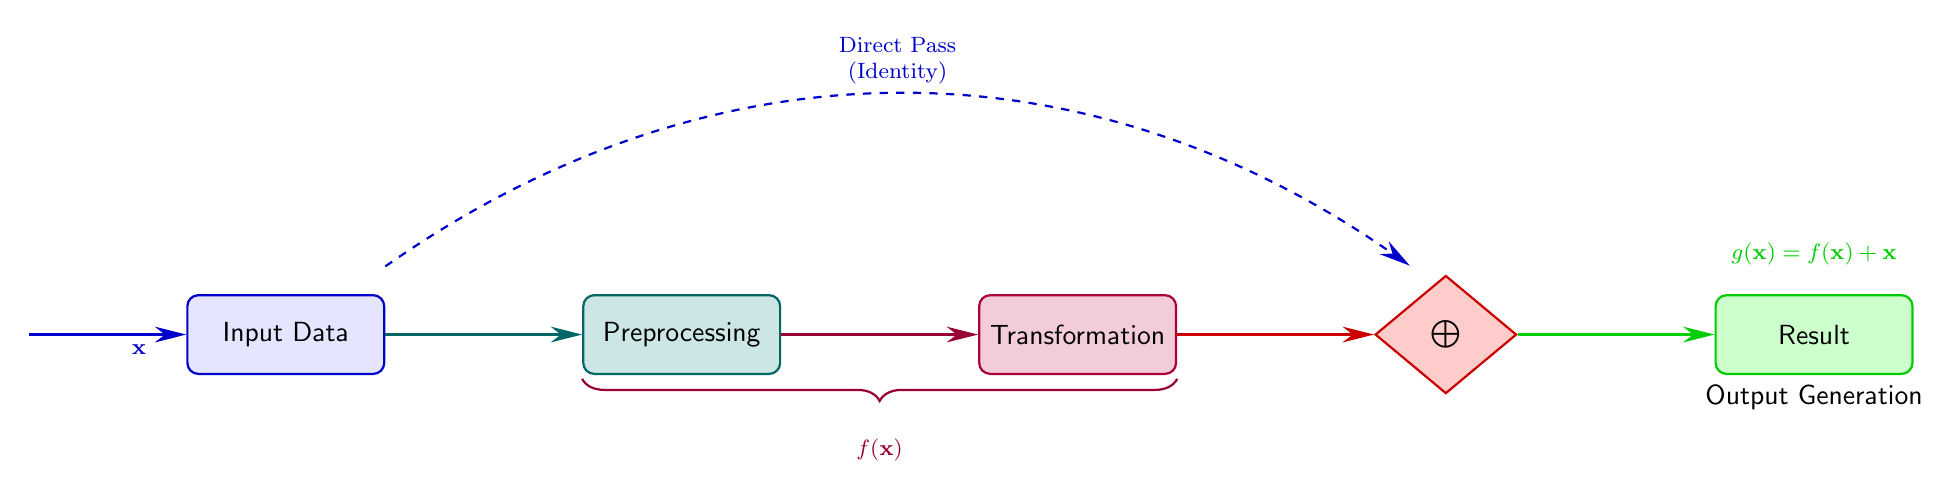
\begin{tikzpicture}[node distance=2.5cm, every node/.style={font=\sffamily}, >=Stealth]

  % Nodes
  \node[rounded corners, draw=blue!80!black, fill=blue!10, thick, minimum width=2.5cm, minimum height=1cm] (input) {Input Data};
  \node[rounded corners, draw=teal!80!black, fill=teal!20, thick, right=of input, minimum width=2.5cm, minimum height=1cm] (preproc) {Preprocessing};
  \node[rounded corners, draw=purple!90!black, fill=purple!20, thick, right=of preproc, minimum width=2.5cm, minimum height=1cm] (trans) {Transformation};
  \node[diamond, draw=red!80!black, fill=red!20, thick, right=of trans, minimum width=1.5cm, minimum height=1.5cm, aspect=2] (merge) {$\bigoplus$};
  \node[rounded corners, draw=green!80!black, fill=green!20, thick, right=of merge, minimum width=2.5cm, minimum height=1cm, label={below:Output Generation}] (output) {Result};

  % Arrows
  \draw[thick, teal!80!black, -{Stealth[length=4mm,width=2mm]}] (input) -- (preproc);
  \draw[thick, purple!80!black, -{Stealth[length=4mm,width=2mm]}] (preproc) -- (trans);
  \draw[thick, red!80!black, -{Stealth[length=4mm,width=2mm]}] (trans) -- (merge);
  \draw[thick, green!80!black, -{Stealth[length=4mm,width=2mm]}] (merge) -- (output);

  % Skip connection
  \draw[thick, blue!80!black, -{Stealth[length=4mm,width=2mm]}, dashed]
    ([yshift=10pt]input.north east) to[bend left=35]
    node[above, midway, font=\footnotesize, align=center, text=blue!80!black] {Direct Pass\\(Identity)} ([yshift=14pt]merge.north west);

  % Input arrow
  \draw[thick, blue!80!black, -{Stealth[length=4mm,width=2mm]}] ([xshift=-2cm]input.west) -- node[below, pos=0.7, font=\footnotesize, text=blue!80!black] {$\mathbf{x}$} (input);

  % Output label
  \node[above=0.25cm of output, font=\footnotesize, text=green!80!black] {$g(\mathbf{x}) = f(\mathbf{x}) + \mathbf{x}$};

  % Decorated brace for transformation
  \draw[decorate, decoration={brace, amplitude=8pt, raise=16pt}, thick, purple!80!black]
    (trans.east) -- node[midway, below=1.2cm, font=\footnotesize, text=purple!80!black] {$f(\mathbf{x})$} (preproc.west);

\end{tikzpicture}
\end{document}